\chapter{Fehlerkorrigierende Codes}

\section{Einführung}

Stellen Sie sich vor, Sie feiern Ihren 18. Geburtstag und wollen ihren besten Freunden einige Fotos aus ihrer Kindheit zeigen. Die Fotos sind aber leider alle verpixelt und können nicht richtig angezeigt werden! Oder stellen Sie sich vor, sie wollen in einigen Jahren Bilder von ihrem Date anschauen, die Bilder auf ihrer Festplatte sind aber alle unleserlich. \textit{Bad luck}? Fast genau dies ist dem Profi-Fotografen Tony Northrup geschehen, als er den 18. Geburtstag seiner Tochter mit Fotos aus deren Kindheit feiern wollte: \href{https://www.youtube.com/watch?v=xvbnhCDfREk}{Video}.

Bei der Übertragung von Bits über das Internet können einzelne Bits spontan verändert oder gelöscht werden -- dies kann fatale Folgen haben! Bei spontaner Änderung von einem 1 zu einem 0 (oder umgekehrt) spricht man von sogenanntem \textit{bit rot}.

\section{Prüfbits}

Buchstaben können auf unterschiedliche Weise kodiert sein -- bei ASCII werden beispielsweise sechs bits pro Zeichen verwendet:

\begin{table}[H]
\centering
\begin{tabular}{c|c}
Buchstabe & Kodierung \\\midrule\midrule
A & 010000001 \\\midrule
B & 010000010\\\midrule
C & 010000011\\\midrule
$\cdots$ & $\cdots$
\end{tabular}
\end{table}
Bei der Datenübertragung können aber einzelne Bits spontan von einem 1 zu einem 0 werden (oder umgekehrt). Was könnte getan werden, um dieser Gefahr vorzubeugen?

Ein erster, einfacher Ansatz bestünde darin, jedem Code noch ein weiteres Bit anzuhängen, so dass die Summe der Bits immer gerade ist:

\begin{table}[H]
\centering
\begin{tabular}{c|c}
Buchstabe & Kodierung \\\midrule\midrule
A & 010000001\textbf{0} \\\midrule
B & 010000010\textbf{0}\\\midrule
C & 010000011\textbf{1}\\\midrule
$\cdots$ & $\cdots$
\end{tabular}
\end{table}

Wenn sich \textit{ein} Bit nun spontan verändert, wird der Code als fehlerhaft erkannt, da die Summe der Bits, welche den Wert 1 haben, nicht mehr gerade ist. Ein Computer könnte nun also anfordern, dass der Code nochmals geschickt wird.

Die Idee von Prüfziffern ist, dass jede Prüfziffer nach dem gleichen Prinzip berechnet ist. Stimmt bei einem erhaltenen Code die Formel mit der Prüfziffer nicht überein, wird der Code als fehlerhaft erkannt.
\begin{myexercise}
Folgende Prüfziffern sind alle nach der gleichen Regel berechnet. Können Sie die Regel erkennen?
\begin{itemize}
\item 31\textbf{6}
\item 1298\textbf{0}
\item 3333574\textbf{2}
\item 2\textbf{8}
\item 10\textbf{9}
\end{itemize}
Was wäre die Kontrollziffer für die Zahl 4163?

\begin{myanswer}
\[3 + 1 + 6 = 10\]
\[1 + 2 + 9 + 8 + 0 = 20\]
\[3 + 3 + 3 + 3 + 5 + 7 + 4 + 2=30\]
etc.
Für die Zahl 4163: 4163\textbf{6}
\end{myanswer}
\end{myexercise}

\subsection{EAN}
Ein EAN bezeichnet einen sogenannten European Article Number. Alle Waren auf dem Markt haben einen solchen Code, welcher aus 13 Ziffern besteht. Häufig wird er in Form eines Strichcodes dargestellt, wobei zwei Striche eine Ziffer darstellen, sowie 2 mal 2 Striche, die den Rand angeben (s. \cref{fig:ean}).

\begin{figure}[H]
\centering
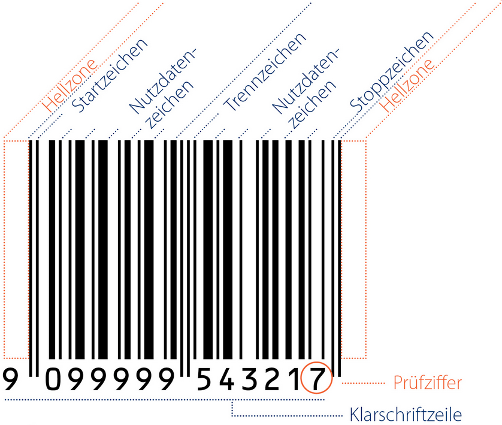
\includegraphics[width=0.7\linewidth]{GrundlagenInfo/05_ErrorChecking/Figures/EAN}
\caption{Bestandteile eines EAN}
\label{fig:ean}
\end{figure}

Ein EAN besteht aus 12 Ziffern und einer Prüfziffer:
\[x_1x_2x_3x_4x_5x_6x_7x_8x_9x_{10}x_{11}x_{12}\textcolor{red}{x_{13}}\]


Das Scannen eines falschen Codes könnte zu falschen Preisen an der Kasse führen, weshalb EAN ebenfalls eine Prüfziffer enthalten.

 die sich wie folgt berechnet:
\begin{enumerate}
\item $s=x_1+x_3+ x_5+ x_7+ x_9+ x_{11}+3\times( x_2+ x_4+ x_6+ x_8+ x_{10}+ x_{12})$
\item Anschliessend wird $\textcolor{red}{x_{13}}$ so gewählt, dass $s+\textcolor{red}{x_{13}}$ durch 10 teilbar ist.
\end{enumerate}


\begin{myexercise}
Welche folgender Fehler werden durch einen EAN erkannt?
\begin{itemize}
\item Vertippen (eine Ziffer ist falsch)
\item Vertauschen zweier benachbarter Ziffern
\item Auslassen (eine Ziffer wird vergessen)
\item 2 mal Vertippen $\rightarrow$ 2 Ziffern werden falsch getippt
\end{itemize}
\end{myexercise}

\begin{myexercise}
Berechnen Sie für 978314221213 die EAN-13-Prüfziffer.
\begin{myanswer}
5
\end{myanswer}
\end{myexercise}

\section{Abstände}

\section{Selbstkorrigierende Codes}

\begin{figure}[H]
\centering
\begin{tikzpicture}
\HyperCube{2}
\end{tikzpicture}
\caption{2D-Hyperwürfel}
\end{figure}

\begin{figure}[H]
\centering
\begin{tikzpicture}
\HyperCube{3}
\end{tikzpicture}
\caption{3D-Hyperwürfel}
\end{figure}




%\only<2-3>{1-Fehler-\textbf{Erkennend}}
%\only<4->{1-Fehler-\textbf{Korrigierend}}
\begin{figure}[H]
\centering
\begin{tikzpicture}
\HyperCube{4}
\end{tikzpicture}
\caption{4D-Hyperwürfel}
\end{figure}

\begin{myexercise}
Zeichnen Sie alle 1-Fehler-erkennenden Kodierungen im unten stehenden Hyperwürfel ein, ausgehend vom Code \texttt{011}.
\begin{figure}[H]
\centering
\begin{tikzpicture}
\HyperCube{3}
% Circle multiple nodes in green
%\only<2->{\CircleNodes{hg-011}}

% Cross out multiple nodes
%\only<3->{\CrossOutNodes{hg-001,hg-010,hg-111}}
%\only<4>{\CircleNodes[green]{hg-101,hg-110,hg-000}}
%\only<4>{\CrossOutNodes{hg-100}}
%\only<5->{\CrossOutNodes{hg-101,hg-000,hg-110}}
%\only<5->{\CircleNodes{hg-100}}

%\CircleNodes[RoyalBlue]{hg-011}
\end{tikzpicture}
\caption{3D-Hyperwürfel}
\end{figure}


\begin{myanswer}

\begin{figure}[H]
\centering
\begin{tikzpicture}
\HyperCube{3}
\CircleNodes{hg-011}

% Cross out multiple nodes
\CrossOutNodes{hg-001,hg-010,hg-111}
\CircleNodes[green]{hg-101,hg-110,hg-000}
\CrossOutNodes{hg-100}
\end{tikzpicture}
\caption{3D-Hyperwürfel}
\end{figure}
\end{myanswer}
\end{myexercise}

\begin{myexercise}
Zeichnen Sie alle 1-Fehler-korrigierenden Kodierungen im unten stehenden Hyperwürfel ein, ausgehend vom Code \texttt{011}.
\begin{figure}[H]
\centering
\begin{tikzpicture}
\HyperCube{3}

\end{tikzpicture}
\caption{3D-Hyperwürfel}
\end{figure}


\begin{myanswer}

\begin{figure}[H]
\centering
\begin{tikzpicture}
\HyperCube{3}
\CircleNodes{hg-011}

% Cross out multiple nodes
\CrossOutNodes{hg-001,hg-010,hg-111}
\CrossOutNodes{hg-101,hg-000,hg-110}
\CircleNodes{hg-100}

%\CircleNodes[RoyalBlue]{hg-011}
\end{tikzpicture}
\caption{3D-Hyperwürfel}
\end{figure}
\end{myanswer}
\end{myexercise}

\begin{myexercise}
Zeichnen Sie alle 1-Fehler-erkennenden Kodierungen im unten stehenden Hyperwürfel ein, ausgehend vom Code \texttt{0000}.
\begin{figure}[H]
\centering
\begin{tikzpicture}
\HyperCube{4}
\end{tikzpicture}
\caption{4D-Hyperwürfel}
\end{figure}


\begin{myanswer}

\begin{figure}[H]
\centering
\begin{tikzpicture}
\HyperCube{4}
\CircleNodes{hg-0000}
\CrossOutNodes{hg-1000,hg-0100,hg-0010,hg-0001}
\CircleNodes[green]{hg-0011,hg-0101,hg-0110,hg-1001,hg-1010,hg-1100,hg-1111}
\CrossOutNodes{hg-0111,hg-1011,hg-1101,hg-1110}
\end{tikzpicture}
\end{figure}
\end{myanswer}
\end{myexercise}

\begin{myexercise}
Zeichnen Sie alle 1-Fehler-korrigierenden Kodierungen im unten stehenden Hyperwürfel ein, ausgehend vom Code \texttt{0000}.
\begin{figure}[H]
\centering
\begin{tikzpicture}
\HyperCube{4}
\end{tikzpicture}
\caption{4D-Hyperwürfel}
\end{figure}

\begin{myanswer}

\begin{figure}[H]
\centering
\begin{tikzpicture}
\HyperCube{4}
\CircleNodes{hg-0000}
\CrossOutNodes{hg-1000,hg-0100,hg-0010,hg-0001}
\CircleNodes[green]{hg-0111}
\CrossOutNodes{hg-0011,hg-0101,hg-0110,hg-1001,hg-1010,hg-1100,hg-1111,hg-1011,hg-1101,hg-1110}
\end{tikzpicture}
\end{figure}
\end{myanswer}
\end{myexercise}


\section{Effiziente Codes}

Error Checking: Ein Zaubertrick \emoji{mage}


$\rightarrow$ Jemand legt ein $n\cdot n$-Grid von Karten aus, einige Karten mit dem Kopf nach oben, andere nach unten (hier: $n=4$):
\begin{figure}[H]
\centering
\AffCartesJeu[Hauteur=1.3,StyleJeu=v1]{DK § Dos § 10T § Dos § 8T}\\
\AffCartesJeu[Hauteur=1.3,StyleJeu=v1]{Dos § AP § AT § VP § Dos}\\
\AffCartesJeu[Hauteur=1.3,StyleJeu=v1]{VT § Dos § 5C § 3T § Dos}\\
\AffCartesJeu[Hauteur=1.3,StyleJeu=v1]{Dos § Dos § 5C § VP § Dos}\\
\end{figure}


$\rightarrow$ Jemand legt nun noch eine weitere Zeile (oben) und eine weitere Spalte (rechts) dazu, ``um das Spiel schwieriger zu machen'':

\begin{figure}[H]
\centering
\AffCartesJeu[Hauteur=1.3,StyleJeu=v1]{Dos § 8C § Dos § VP § 8P § 6C}\\
\AffCartesJeu[Hauteur=1.3,StyleJeu=v1]{DK § Dos § 10T § Dos § 8T § RT}\\
\AffCartesJeu[Hauteur=1.3,StyleJeu=v1]{Dos § AP § AT § VP § Dos § VC}\\
\AffCartesJeu[Hauteur=1.3,StyleJeu=v1]{VT § Dos § 5C § 3T § Dos § 7K}\\
\AffCartesJeu[Hauteur=1.3,StyleJeu=v1]{Dos § Dos § 5C § VP § Dos § Dos}\\
\end{figure}



Anschliessend dreht jemand eine Karte um. Welche war es?
\begin{figure}[H]
\centering
\AffCartesJeu[Hauteur=1.3,StyleJeu=v1]{Dos § 8C § Dos § VP § 8P § 6C}\\
\AffCartesJeu[Hauteur=1.3,StyleJeu=v1]{DK § Dos § 10T § Dos § 8T § RT}\\
\AffCartesJeu[Hauteur=1.3,StyleJeu=v1]{Dos § AP § AT § VP § Dos § VC}\\
\AffCartesJeu[Hauteur=1.3,StyleJeu=v1]{VT § Dos § Dos § 3T § Dos § 7K}\\
\AffCartesJeu[Hauteur=1.3,StyleJeu=v1]{Dos § Dos § 5C § VP § Dos § Dos}\\
\end{figure}

Gerade Zahlen spalten- und zeilenweise summieren:
\begin{itemize}
\item Zeilen: 4, 4, 4, \textbf{3}, 2
\item Spalten: 2, 2, \textbf{3}, 4, 2, 4
\end{itemize}
